\documentclass[11pt,aspectratio=169,dvipsnames]{beamer}
\graphicspath{{figs/}}
\usetheme{default}
\usepackage{DasBeamerPaket}
\usepackage{animate}
\usepackage{lastpage}
%\usepackage{enumitem}
\usepackage{appendixnumberbeamer}
\usepackage{braket}
\usepackage{tikz}
\setbeamercolor{section in toc}{fg=NavyBlue}
\setbeamercolor{frametitle}{fg=NavyBlue}
\captionsetup[figure]{labelfont=bf}
\captionsetup[table]{labelfont=bf}
\newcommand{\theauthor}{Jakob Krause}
\newcommand{\theshortauthor}{\textsc{J. Krause} for CBELSA/TAPS}
\newcommand{\authormail}{krause@hiskp.uni-bonn.de}
\newcommand{\authorgit}{krausejm}
\newcommand{\thetitle}{Recent Polarization Observable Results in  $\eta$- and $\eta'$-photoproduction off the proton}
\newcommand{\theshorttitle}{$\Sigma$ in $\eta$- and $\eta'$ photoproduction}
\newcommand{\thecolor}{black!70!blue}
\newcommand{\thecolorr}{black!60!blue}
\newcommand{\thecolorrr}{black!50!blue}
\newcommand{\thesubtitle}{Master thesis for the CBELSA/TAPS collaboration}
\newcommand{\thedate}{30th March 2022}
\makeatletter
\patchcmd{\beamer@calculateheadfoot}{\advance\footheight by 4pt}{\advance\footheight by 20pt}{}{}
\makeatother
\begin{document}
	\definecolor{myWhite}{rgb}{1,1,1}
	
	
	\setbeamercolor{coloredboxstuff}{fg=myWhite,bg=\thecolor}
	\setbeamercolor{coloredboxstuff1}{fg=myWhite,bg=\thecolorr}
	\setbeamercolor{coloredboxstuff2}{fg=myWhite,bg=\thecolorrr}	
	\makeatother
	\setbeamertemplate{footline}
	{
		\leavevmode%
		\hbox{%
			\begin{beamercolorbox}[wd=.33\paperwidth,ht=2.25ex,dp=1ex,center]{coloredboxstuff}%
				{\theshortauthor}
			\end{beamercolorbox}%
			\begin{beamercolorbox}[wd=.34\paperwidth,ht=2.25ex,dp=1ex,center]{coloredboxstuff1}%
				{\theshorttitle}
			\end{beamercolorbox}%
			\begin{beamercolorbox}[wd=.33\paperwidth,ht=2.25ex,dp=1ex,center]{coloredboxstuff}%
				\insertframenumber{} / \inserttotalframenumber\hspace*{1ex}
		\end{beamercolorbox}}%
	}
	\makeatletter
	
	
	\setbeamercovered{transparent}
	\setbeamertemplate{navigation symbols}{}
	\setbeamertemplate{frametitle}[default][left,leftskip=0.5cm]
	\setbeamertemplate{itemize item}{\color{black}$\blacktriangleright$}
	\setbeamertemplate{section in toc}[sections numbered]
	\setbeamercolor{section in toc}{fg=\thecolor}
	\setbeamercolor{frametitle}{fg=\thecolor}
	\captionsetup{font=scriptsize,labelfont=scriptsize}
	\AtBeginSection[]
	{	
		
		{
			
			\makeatother
			\setbeamertemplate{footline}
			{
				\leavevmode%
				\hbox{%
					\begin{beamercolorbox}[wd=.34\paperwidth,ht=2.25ex,dp=1ex,center]{coloredboxstuff}%
						{|\hfill\theshortauthor\hfill|}
					\end{beamercolorbox}%
					\begin{beamercolorbox}[wd=.34\paperwidth,ht=2.25ex,dp=1ex,center]{coloredboxstuff}%
						{\theshorttitle}
					\end{beamercolorbox}%
					\begin{beamercolorbox}[wd=.34\paperwidth,ht=2.25ex,dp=1ex,center]{coloredboxstuff}%
						\insertsection\hspace*{1ex}
				\end{beamercolorbox}}%
			}
			\makeatletter
			
			
			\begin{frame}[noframenumbering]
				\frametitle{}
				\addtocounter{page}{-1}
				\tableofcontents[currentsection]
			\end{frame}
		}
		
	}
	%\begin{frame}[plain]
	%	\centering
	%	{\Large \color{\thecolor}{\thetitle}}\\
	%	\vspace{0.5cm}
	%	{\thesubtitle}
	%	\vfill
	%	\begin{minipage}{\linewidth}
		%		\centering
		%		\begin{minipage}{\linewidth}
			%			\textsc{\theauthor}\\
			%			\scriptsize \href{mailto:\authormail}{\faEnvelope  \hspace*{0.1cm}\authormail} {\color{black}$|$} \href{https://github.com/\authorgit}{\faGithub  \hspace*{0.1cm}\authorgit}\\
			%		\end{minipage}
		%		\vspace{.5cm}
		
		%		{\scriptsize
			%			Supervisor: \textsc{Jun. Prof. Dr. Annika Thiel}\\
			%			\tiny \href{mailto:thiel@hiskp.uni-bonn.de}{\faEnvelope  \hspace*{0.1cm}thiel@hiskp.uni-bonn.de}\par}
		%	\end{minipage}
	%	\vspace{0.2cm}
	
	%	\thedate
	%\end{frame}
	
\begin{frame}{Event selection of $\eta'\to\gamma\gamma$}
	\begin{itemize}
		\item background contributions from $2\pi^0,\pi^0\eta$, $\frac{N_{2\pi^0}}{N_{\eta'}}=\frac{\sigma_{2\pi^0}\cdot\text{BR}(2\pi^0\to4\gamma)}{\sigma_{\eta'}\cdot\text{BR}(\eta'\to\gamma\gamma)}\approx\frac{5\si{\micro\barn}\cdot0.98}{1\si{\micro\barn}\cdot0.02}=245$\\
		$\frac{N_{\pi^0\eta}}{N_{\eta'}}=\frac{\sigma_{\pi^0\eta}\cdot\text{BR}(\pi^0\eta\to4\gamma)}{\sigma_{\eta'}\cdot\text{BR}(\eta'\to\gamma\gamma)}\approx\frac{3\si{\micro\barn}\cdot0.38}{1\si{\micro\barn}\cdot0.02}=57$
		
		\item cuts (proton in MT, clustersizes, energy of photons) may reduce $2\pi^0,\pi^0\eta$ contributions but NOT within cut ranges..
		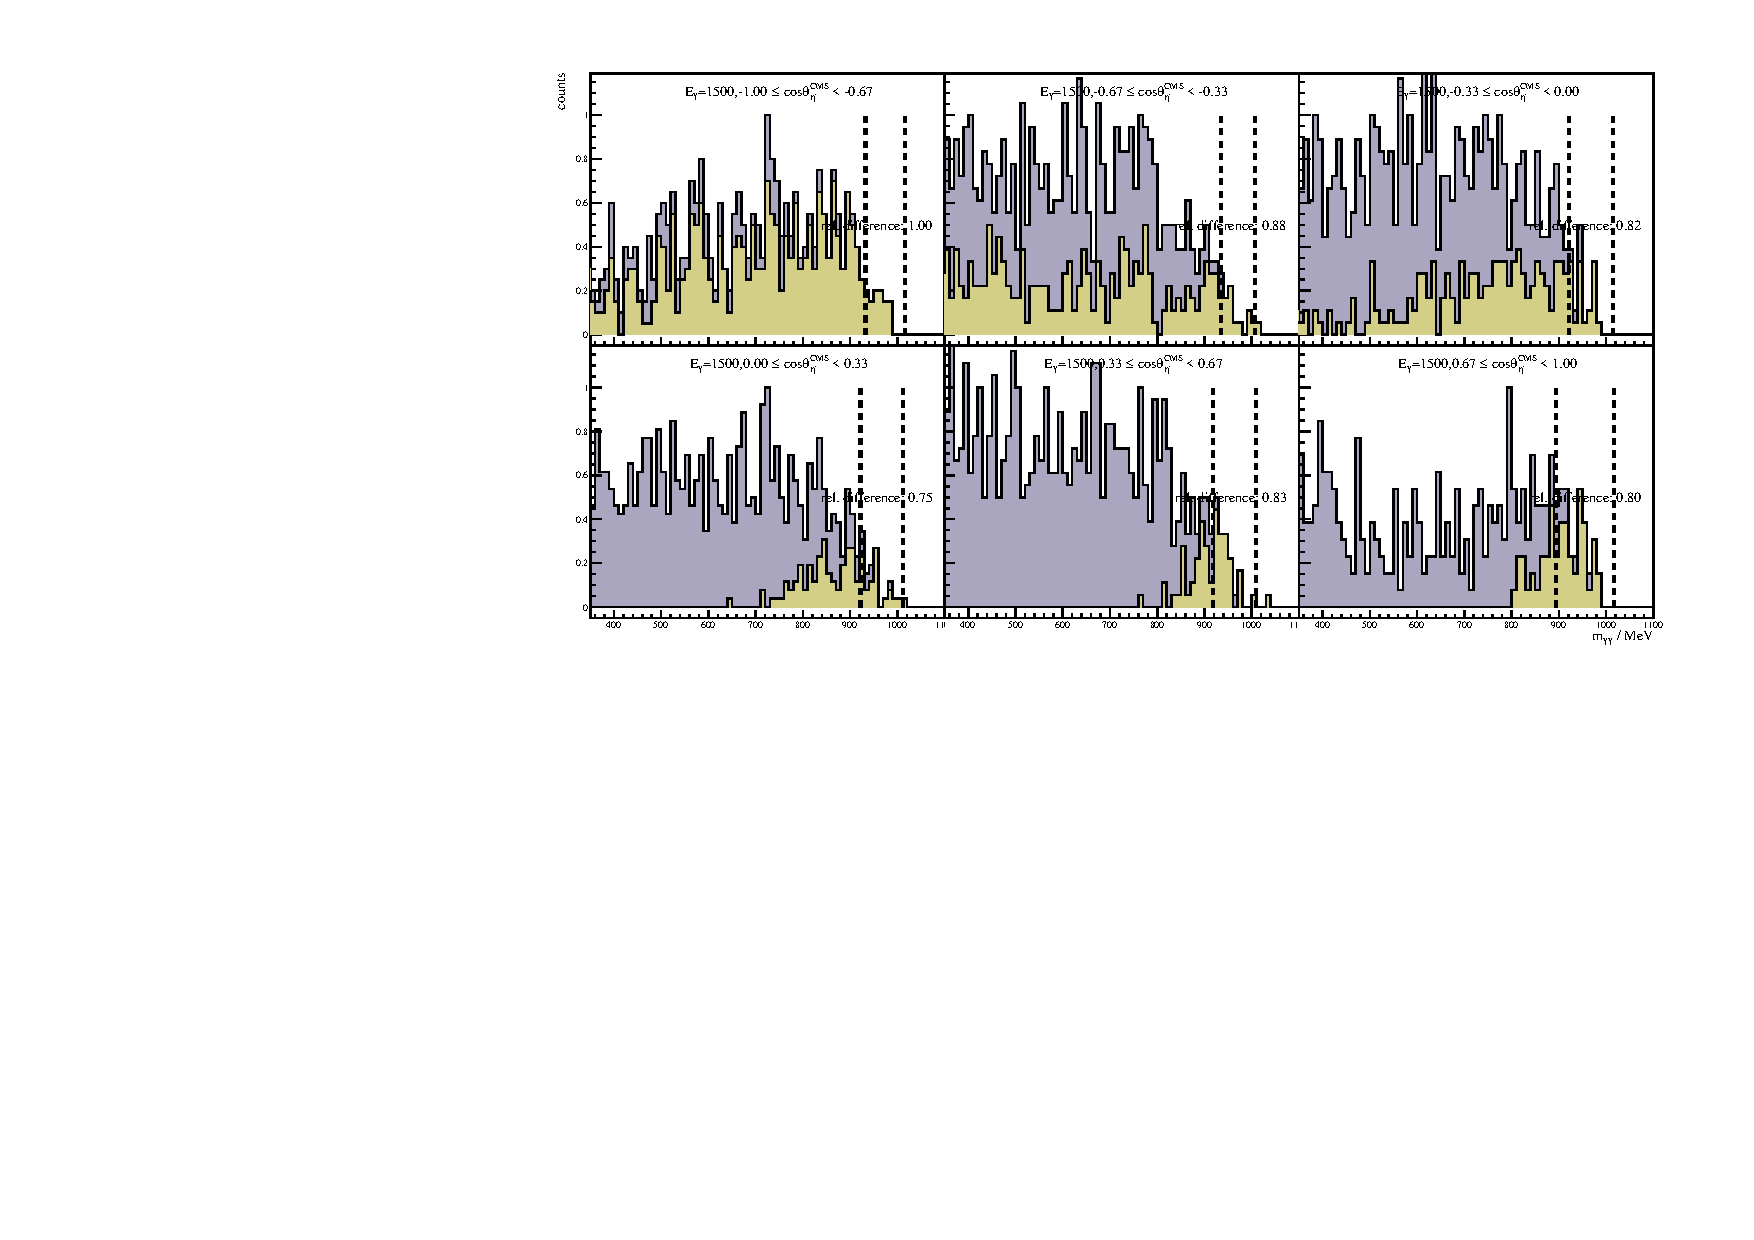
\includegraphics[width=.6\columnwidth]{../../figs/hydrogen/allcuts_2pi0.pdf}
		\item $\to$ keep bkg for a better MC fit, use PWA MC for better fit
	\end{itemize}
\end{frame}
\begin{frame}{Event selection of $\eta'\to\gamma\gamma$}
	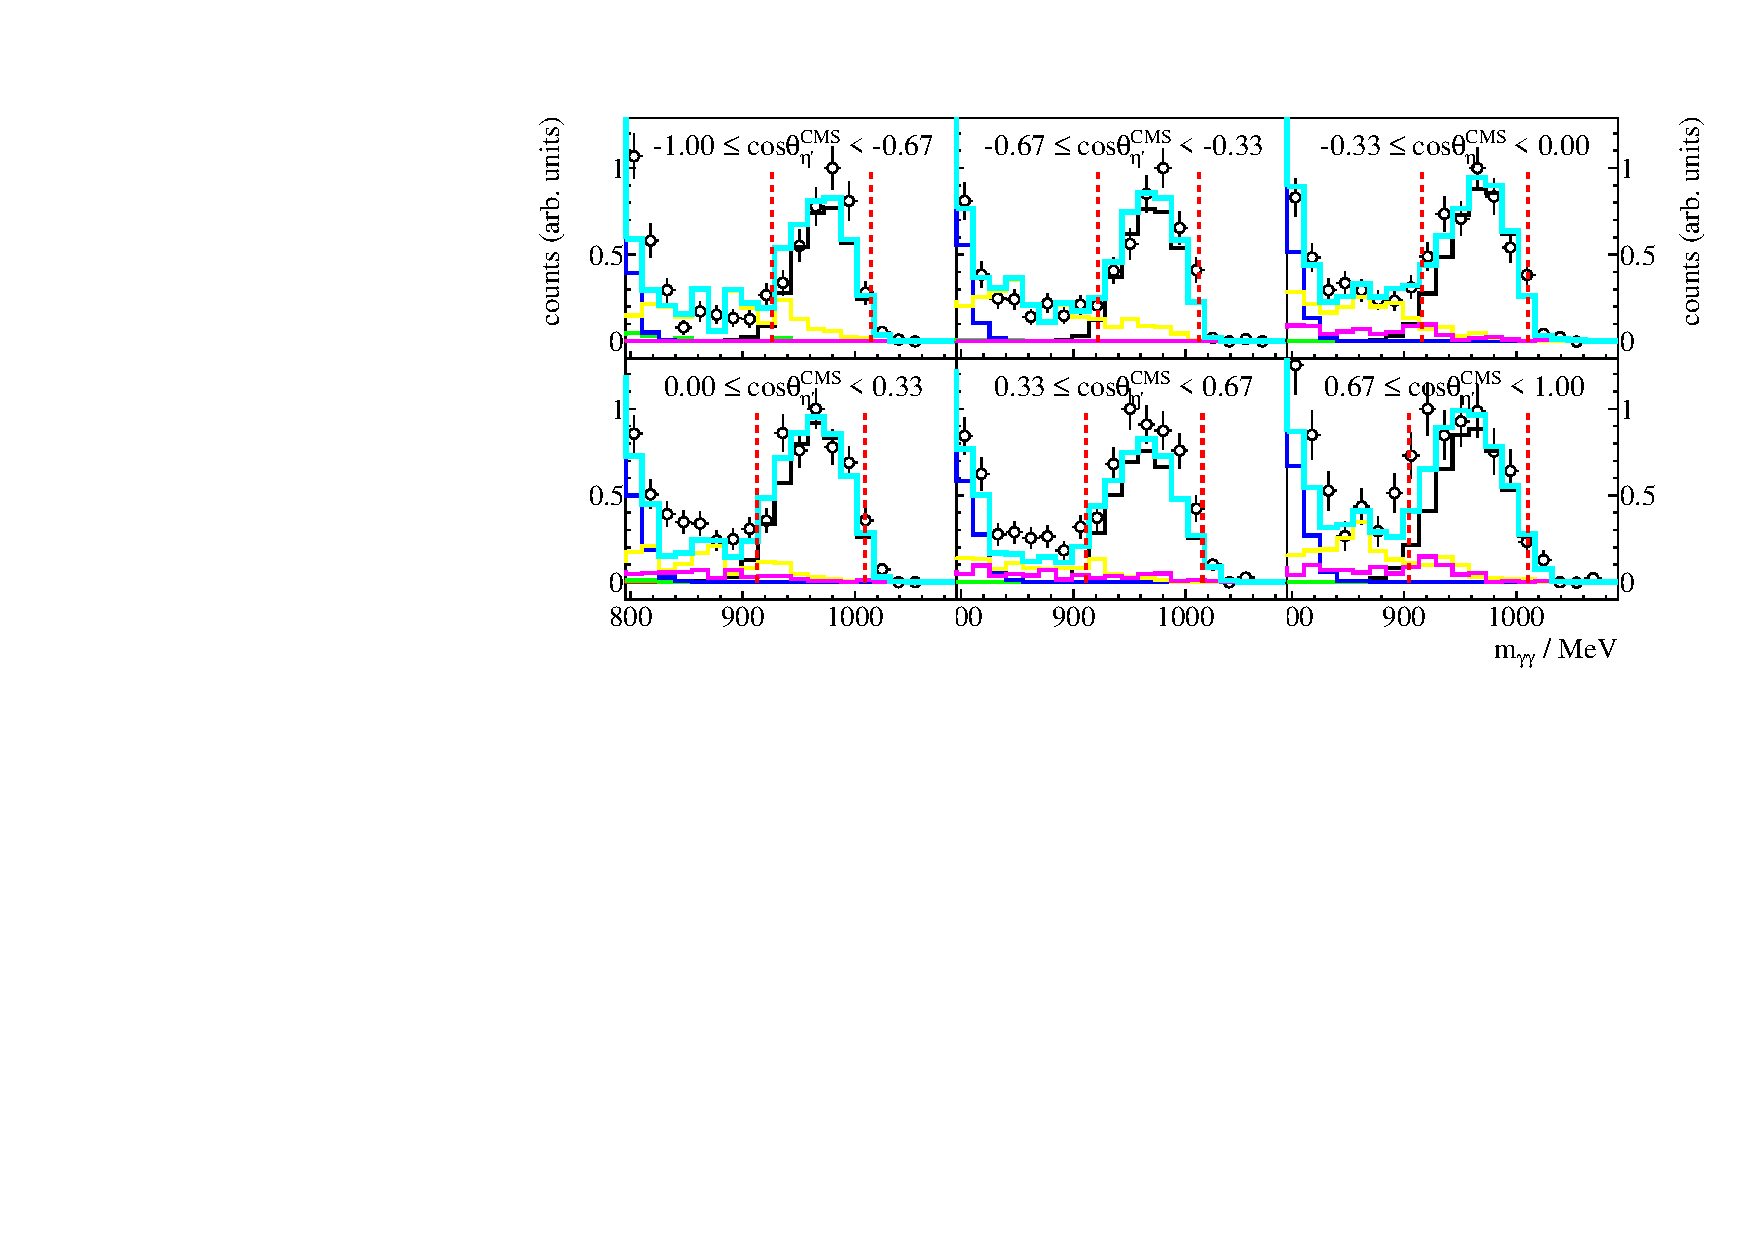
\includegraphics[width=.49\linewidth]{../../figs/hydrogen/bin_cuts/invcut_ebin1.pdf}
	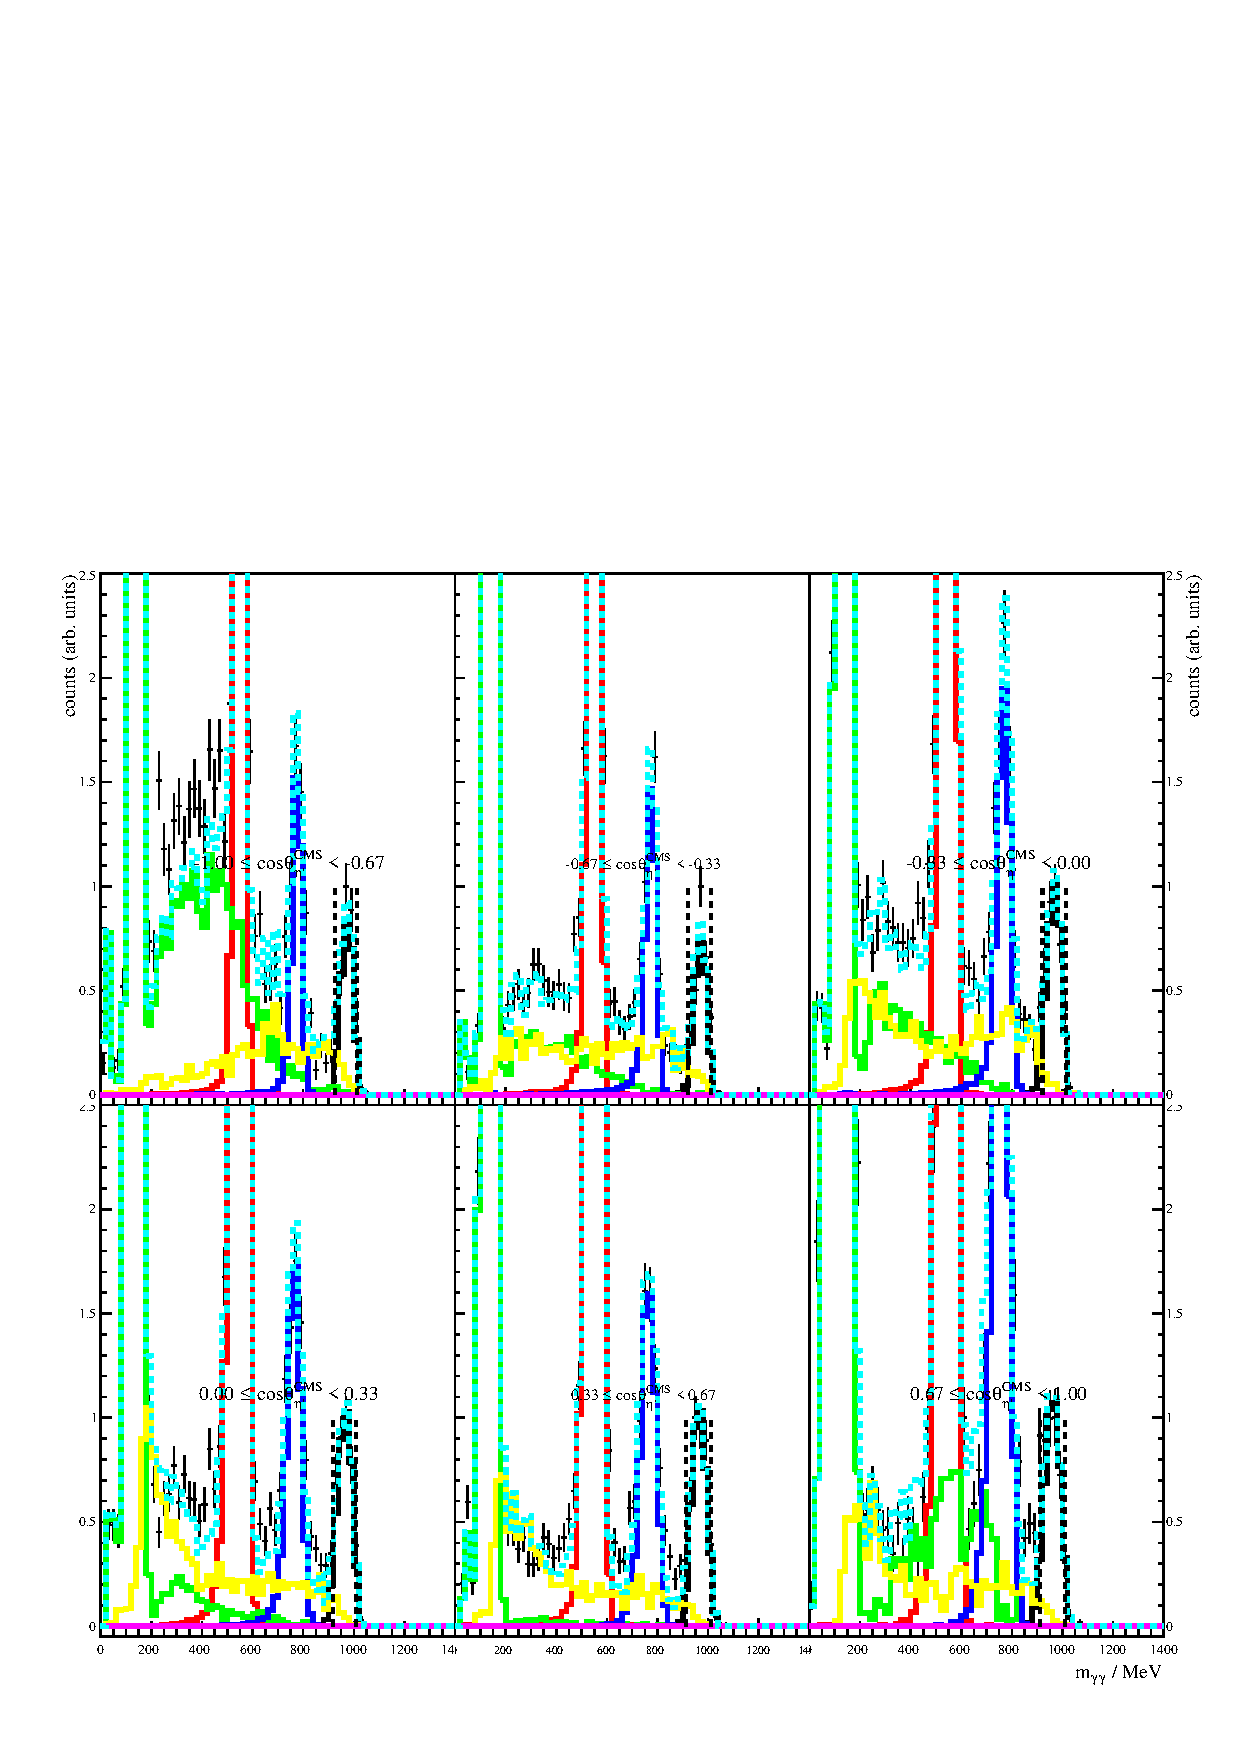
\includegraphics[width=.49\linewidth]{../../figs/hydrogen/bin_cuts/invcut_ebin1_only2pi0.pdf}
	$\to$ treat $2\pi^0$ contributions rigorously and $\pi^0\eta$ as systematical error (?)
\end{frame}
\begin{frame}{Event selection of $\eta'\to\gamma\gamma$}
	\centering	
	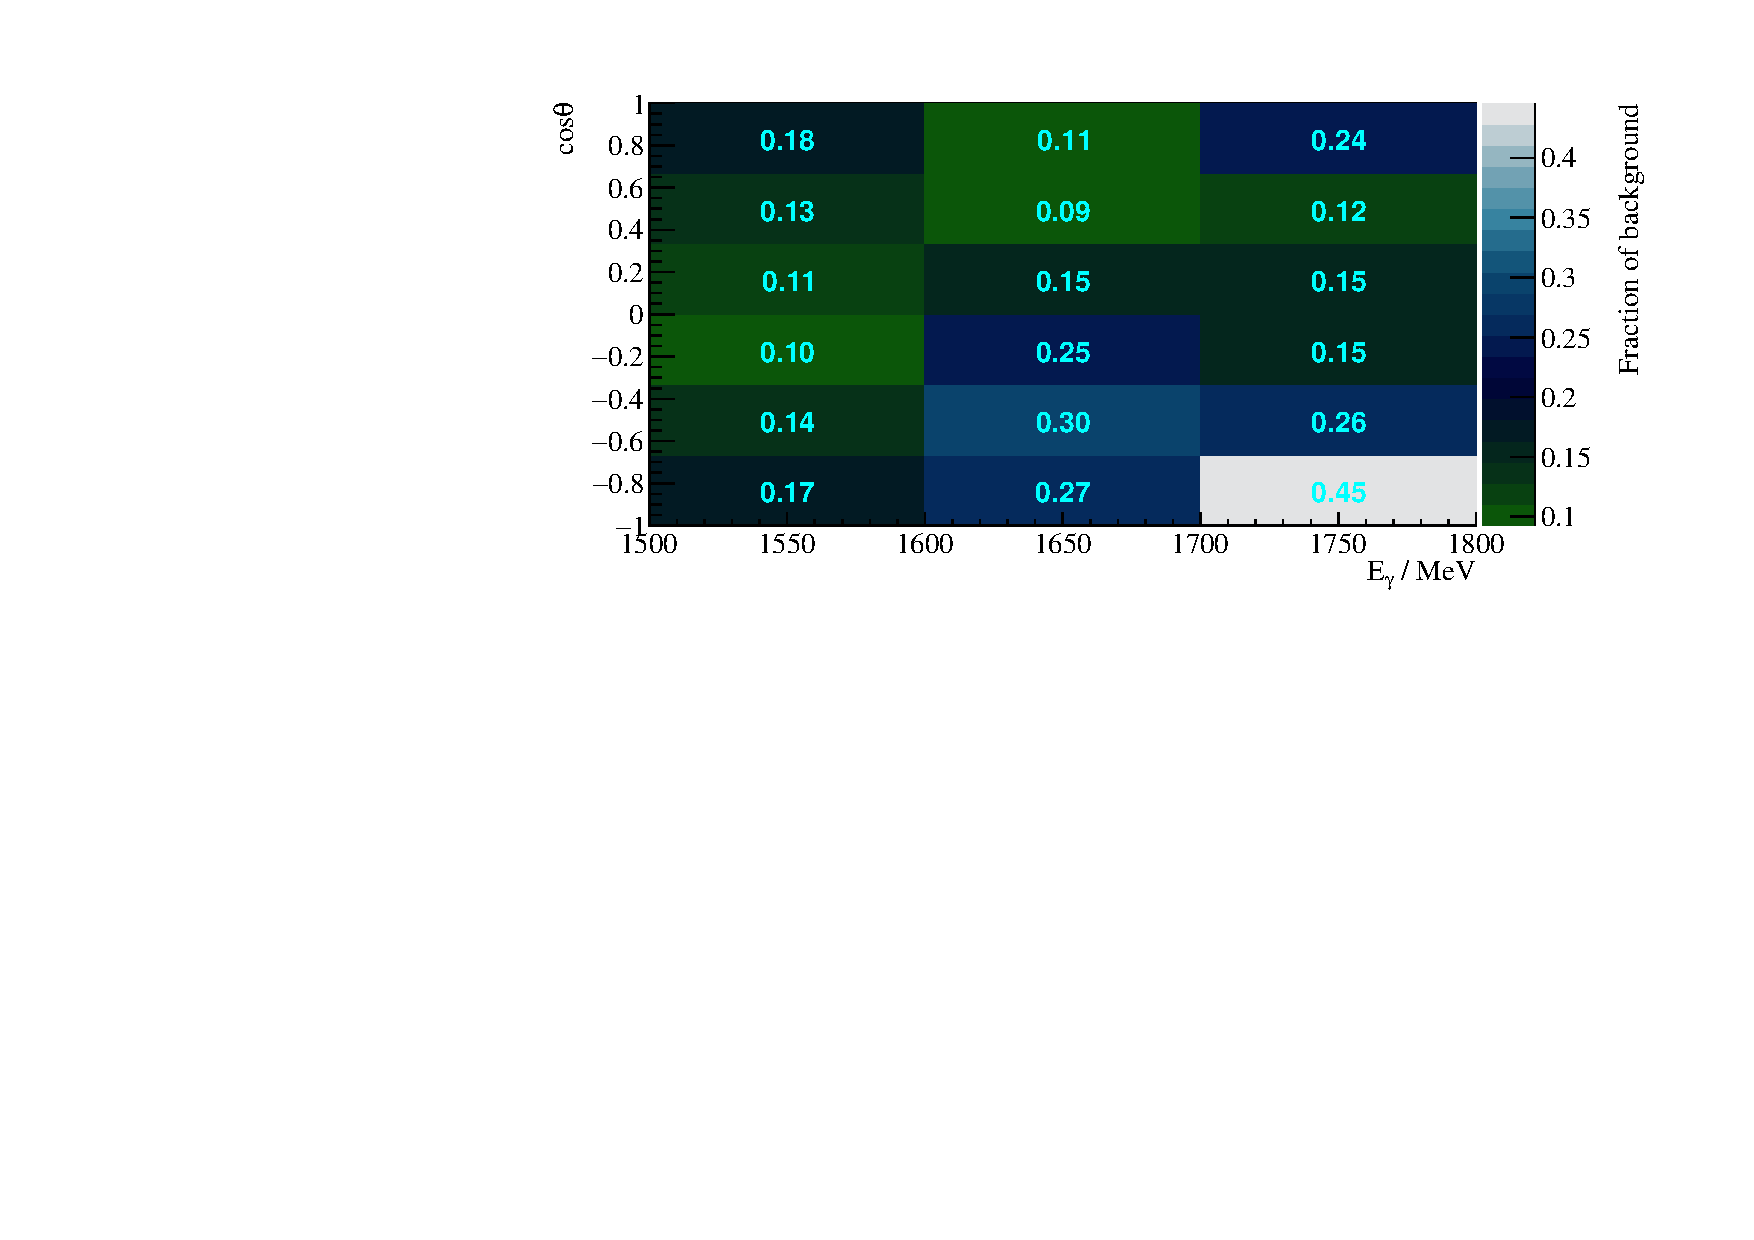
\includegraphics[width=.7\linewidth]{../../figs/hydrogen/bin_cuts/invcut_bkg_percentage.pdf}\\
	$\to$ unbinned fits (Bayes and RooFit) $\Sigma=a\cdot\Sigma_{\eta'}+b\cdot\Sigma_{2\pi^0}$
\end{frame}
\begin{frame}{Binned fits for $\eta\to\gamma\gamma$ toy MC}
\begin{table}[]
	\begin{tabular}{cccccc}
		nbins & chi2    & abserror    & abserror\_err & sigma\_std & mean\_sigma\_err \\
		\hline
		5     & 1.0084  & -0.136562   & 0.0106015     & 0.122244   & 0.115216         \\
		10    & 1.01608 & -0.0807627  & 0.00745136    & 0.122413   & 0.116159         \\
		15    & 1.0213  & -0.0453879  & 0.0060793     & 0.122955   & 0.116755         \\
		20    & 1.02628 & -0.0204121  & 0.00526841    & 0.123345   & 0.117157         \\
		25    & 1.03135 & -0.00104504 & 0.00472013    & 0.123842   & 0.117438         \\
		30    & 1.03643 & 0.0154211   & 0.00432156    & 0.124417   & 0.117639         \\
		35    & 1.04177 & 0.0308903   & 0.00401215    & 0.124929   & 0.117784         \\
		40    & 1.04692 & 0.0448043   & 0.00376464    & 0.125443   & 0.117886         \\
		45    & 1.05254 & 0.0575842   & 0.0035624     & 0.12597    & 0.117957         \\
		50    & 1.05817 & 0.0700262   & 0.00339457    & 0.126521   & 0.118002         \\
		55    & 1.06402 & 0.0818481   & 0.00325091    & 0.127102   & 0.118027         \\
		60    & 1.07006 & 0.09364     & 0.00312813    & 0.127734   & 0.118034         \\
		65    & 1.07618 & 0.105762    & 0.00302238    & 0.128386   & 0.118028         \\
		70    & 1.08248 & 0.117378    & 0.00292896    & 0.129054   & 0.118009         \\
		75    & 1.08918 & 0.129015    & 0.00284671    & 0.129795   & 0.11798          \\
		80    & 1.09582 & 0.140795    & 0.00277291    & 0.130517   & 0.117942         \\
		85    & 1.10262 & 0.152683    & 0.00270763    & 0.131278   & 0.117896         \\
		90    & 1.10958 & 0.164707    & 0.00264856    & 0.13206    & 0.117842         \\
		95    & 1.11669 & 0.176578    & 0.00259558    & 0.132879   & 0.117782         \\
		100   & 1.11669 & 0.172502    & 0.00253218    & 0.147134   & 0.117782        
	\end{tabular}
\end{table}
\end{frame}
	

	
\end{document}
